\documentclass[10pt,oneside]{article}
\usepackage[utf8]{inputenc}
\usepackage[T1]{fontenc}
\usepackage{latexsym}
\usepackage[spanish,es-nodecimaldot,es-noshorthands]{babel}
\usepackage{amsfonts}
\usepackage{multicol}
\usepackage{amsmath}
\usepackage{amssymb}
\usepackage{amsthm}
\usepackage[all]{xy}
\usepackage{tikz}
\usepackage[retainorgcmds]{IEEEtrantools}
\usepackage{mathrsfs}
\usepackage{ upgreek }
\usepackage{tcolorbox}
\tcbuselibrary{theorems}
\usepackage[pdftex]{hyperref}
\addtolength{\hoffset}{-3.5cm}
\addtolength{\textwidth}{7.2cm}
\addtolength{\voffset}{-3cm}
\addtolength{\textheight}{5cm}
\pagestyle{empty}


\title{\textbf{Notas de Modelación Epidemiológica}}

\author{Lucho Cervantes Jorge Luis}


\begin{document}

\maketitle

\begin{multicols}{2}

    \section{Introducción}
    
    \textbf{Epidemiología:} Estudio de una población respecto a su estado de salud. Para esto se definen clases epidemiológicas. La unión de estas clases es resulta en la población. \\ \newline \textbf{Estado de salud:} Según la OMS, estado de bienestar fisiológico, psicológico y social. \\ \newline Se tiene un enfoque en enfermedades causadas por patógenos como virus, bacterias, hongos, priones, etc.
    \textbf{Herramientas matemáticas:}
    
    \begin{enumerate}
        \item \textbf{Estadística}
        \begin{itemize}
            \item Muestreo: cuando el tamaño de muestra es suficientemente grande para hacer buenas predicciones.
            \item Inferencias:
            \begin{itemize}
                \item[*] bayesianas
                \item[*] frecuentistas
            \end{itemize}
        \end{itemize}
        \item \textbf{Azar}: si los datos no son suficientes se puede hacer una aproximación y/o ajuste de datos aleatorios o con una distribución que corresponda con las observaciones. Esto implica cierto grado de incertidumbre (Procesos estocásticos).
        \item \textbf{Aproximaciones de campo medio}: a partir de estas se aplican las ecuaciones diferenciales de la forma:
        $$\frac{dS}{dt}=-\alpha SI+ f(S,I;...)$$
        donde el término $SI$ es no lineal y en general es el que mide cómo interaccionan los individuos de una clase epidemiológica con los de otra. \\ \newline En este caso $S$ es la población susceptible o (saludable) e $I$ es la población infectada. En este tipo de modelos se hace la \textit{hipótesis de la buena mezcla}, i.e. que todos los individuos de $S$ tienen la misma probabilidad de infectarse al contactar un elemento de $I$. Esto no es necesariamente cierto.
        \item \textbf{Redes:} se utilizan para tomar en cuenta las inhomogeneidades que pueden presentar las poblaciones mediante pesos de las conexiones de sus nodos.
        \item \textbf{Herramientas computacionales:}
        \begin{itemize}
            \item Autómatas celulares: abarca la espacialidad y el comportamiento local de los individuos.
            \item Modelos multi agentes: abarca el comportamiento (Problema de la racionalidad acotada).
        \end{itemize}
    \end{enumerate}
    
    \textbf{Enfermedades}
    
    \begin{enumerate}
        \item \textbf{Infecciosas} (patógenos)
        \begin{itemize}
            \item comunicables: se transmiten de persona a persona por contacto directo 
            \item Transmitibles: se transmiten de persona a persona, pero puede ser por vía aérea, por comida infectada, el agua. También enfermedades vectoriales (una persona infecta algún vector, como el mosquito en el dengue, y este a su vez infecta a otra persona) y enfermedades verticales (las que se heredan). 
        \end{itemize} 
        \item \textbf{Sistémicas:} Como la diabetes.
    \end{enumerate} 
    
    Términología que se utiliza respecto al \textbf{estado de la enfermedad}.
    
    \begin{enumerate}
        \item \textbf{Expuesto}: contacto efectivo con un infectado.
        \item \textbf{Infectado}: Si el patógeno se establece en el cuerpo de alguien expuesto. 
        \item \textbf{Infeccioso}: infectado que puede contagiar.
        \item \textbf{Latente}: infectado que no puede contagiar, al menos, por un tiempo (tiempo de latencia).
        \item \textbf{Incubación}: Periodo entre la exposición y la infección.
        \item \textbf{Prevalencia}: Número de infectados en un tiempo específico.
        \item \textbf{Incidencia}: Número de infectados en un intervalo de tiempo.
        \item \textbf{Fatalidad}: Número de muertos por la enfermedad respecto al número de infectados.
        \item \textbf{Mortalidad}: Número de muertos por la enfermedad respecto a la población total.
    \end{enumerate}

    \section{Modelo de Kermack-McKendrick (SIR)}

    Considera enfermedades que se transmiten por contacto, periodo de incubación pequeño, tasa de mortalidad baja, tasa de contagio "alta", duración corta y que genera inmunidad.\\ \newline Se considera la parte de la población susceptible, $S$, la parte infectada, $I$ y la parte removida, $R$, (muertos y recuperados que adquieren inmunidad permanente). Modela, por ejemplo, la varicela y el sarampión de manera aproximada.\\ \newline \textbf{Hipótesis:}

    \begin{itemize}
        \item No hay efectos demográficos debido a la escala de tiempo de la enfermedad (No se consideran los nacimientos ni las muertes naturales).
        \item Población cerrada (No hay efectos de migración).
        \item Población bien mezclada (Toda la población tiene la misma probabilidad de tener un contacto efectivo con un infectado y la misma probabilidad de infectarse).
        \item Inmunidad permanente (Los removidos no infectan).
    \end{itemize}

    La población total, $N$, al tiempo, $t$, es tal que:
    
    \begin{equation}\label{eq:1}
        N(t)=S(t)+I(t)+R(t),
    \end{equation}
    
    donde $cN$ es el contacto efectivo por unidad de tiempo y $S/N$ es la probabilidad de contacto. Entonces, $cN\cdot S/N=cS$ es el contacto efectivo. Definiendo $P$ como la probabilidad de transmisión y $\beta=Pc$ se tiene que la probabilidad de que una persona se infecte es $cS\cdot P=\beta S$. En consecuencia, la tasa de infectados infecciosos es $cSI$. \\ \newline El modelo se representa con el diagrama:
    \begin{center}\vspace{0.3cm}
       \hspace{0.6cm}\xymatrix{*+<0.6cm>[F]{S} \ar[r]^{\beta I} & *+<0.6cm>[F]{I} \ar[r]^{\alpha}&*+<0.6cm>[F]{R}} 
       \vspace{0.3cm}
    \end{center} Donde se expresa que $I$ depende de $\beta S$ y $R$ de la tasa de remoción $\alpha$. El modelo es:

    \begin{equation}\label{eq:2}
         \tcboxmath[colback=white,colframe=gray, title=Modelo de Kermack-McKendrick (SIR)]{\begin{array}{ccl}
            \dot S & = & -\beta SI \\
            \dot I & = & \beta SI - \alpha I\\
            \dot R & = & \alpha I\\
        \end{array}} 
    \end{equation}
    % Para hacer las cajitas de colores solo se requieren  \usepackage{tcolorbox} y \tcbuselibrary{theorems}.
    
    con las condiciones iniciales $S(0)=S_0$, $I(0)=I_0$ Y $R(0)=0$ ($\Rightarrow N_0=R_0+S_0$). En particular 

    \begin{equation}\label{eq:3}
        \dot N=\dot S+\dot I+\dot R\equiv 0; \hspace{0.5cm} N\equiv0. 
    \end{equation}
    
    Considerando:
    
    $$\lim_{t \to\infty }=S_{\infty},$$ $$\lim_{t\to\infty }=I_{\infty},$$ $$\lim_{t\to\infty }=R_{\infty}$$ 
    
    también se tiene que:

    \begin{equation}\label{eq:4}
        N=S_{\infty}+R_{\infty}.
    \end{equation}

    Cuando $I>S$ se dice que hay una epidemia. Para que la población infectada aumente se tiene que: 

    $$\dot I(t)>0\hspace{0.5cm} \forall t$$ $$\Leftrightarrow \hspace{0.5cm}\dot I(t=0)=(\beta S_0-\alpha) I_0>0$$ $$\Leftrightarrow\hspace{0.5cm} \frac{\beta}{\alpha}S_0>1$$

    A $R_0 \equiv\beta S_0/\alpha $ se le conoce como número de reproducción básico y puede pensarse como el número de casos secundarios que produce un único infeccioso en la población susceptible. Si $R_0>1$ hay brote epidémico. Si $R_0\leq1$ no hay brote epidémico. \\ \newline
    Por otro lado, la tercera ecuación de (\ref{eq:2}) es redundante pues $\dot R=\alpha I$ aparece  en la segunda ecuación. Así, el sistema puede resolverse considerando solo las primeras dos ecuaciónes y que 
    
     \begin{equation}\label{eq:5}
         R(t)=\underbrace{N}_{\textnormal{cte.}}-S(t)-I(t).
     \end{equation}

     Comparando $S$ con $R$:

     $$\frac{dS}{dR}=\frac{\frac{dS}{dt}}{\frac{dR}{dt}}=\frac{\dot S}{\dot R}=-\frac{\beta SI}{\alpha I}=-\frac{\beta S}{\alpha}$$ $$\Rightarrow\hspace{0.5cm} S(t)=S_0 e^{\frac{\beta}{\alpha} R}.$$

     Comparando $S$ con $I$:

      $$\frac{dS}{dI}=-\frac{\beta SI}{\beta SI-\alpha I}=-\frac{\beta S}{\beta S-\alpha }$$
      $$\Leftrightarrow\hspace{0.5cm}\int \frac{\alpha-\beta S}{\beta S}dS=\int dI =I$$
      $$\Leftrightarrow\hspace{0.5cm}\int \frac{\alpha-\beta S}{\beta S}dS=\int dI =I$$
      $$\Leftrightarrow\hspace{0.5cm}I=\frac{\alpha}{\beta}\int\frac{dS}{S}-\int dS=\frac{\alpha}{\beta}\ln S-S$$
      $$\Leftrightarrow\hspace{0.5cm} I+S-\frac{\alpha}{\beta}\ln S=\textnormal{cte.} \hspace{0.5cm} \forall t$$

      Para $t=0$
      
      $$\Leftrightarrow\hspace{0.5cm} \underbrace{S_0+I_0}_{=N}-\frac{\alpha}{\beta}\ln S_0= \textnormal{cte.}$$

      Para $t\to \infty$

      $$\Leftrightarrow\hspace{0.5cm} S_{\infty}+\underbrace{I_{\infty}}_{=0}-\frac{\alpha}{\beta}\ln S_{\infty}= \textnormal{cte.}$$

      Entonces:

      $$N-S_{\infty}=\frac{\alpha}{\beta}(\ln S_0-\ln S_{\infty})=\frac{\alpha}{\beta}\ln \frac{S}{S_{\infty}} $$
      $$ \Rightarrow \frac{\beta}{\alpha}=\frac{\ln \frac{S}{S_{\infty}}}{N-S_{\infty}} $$

      La figura \ref{fig:1} Muestran el comportamiento dede las soluciones.
      
      \begin{figure*}
          \centering
          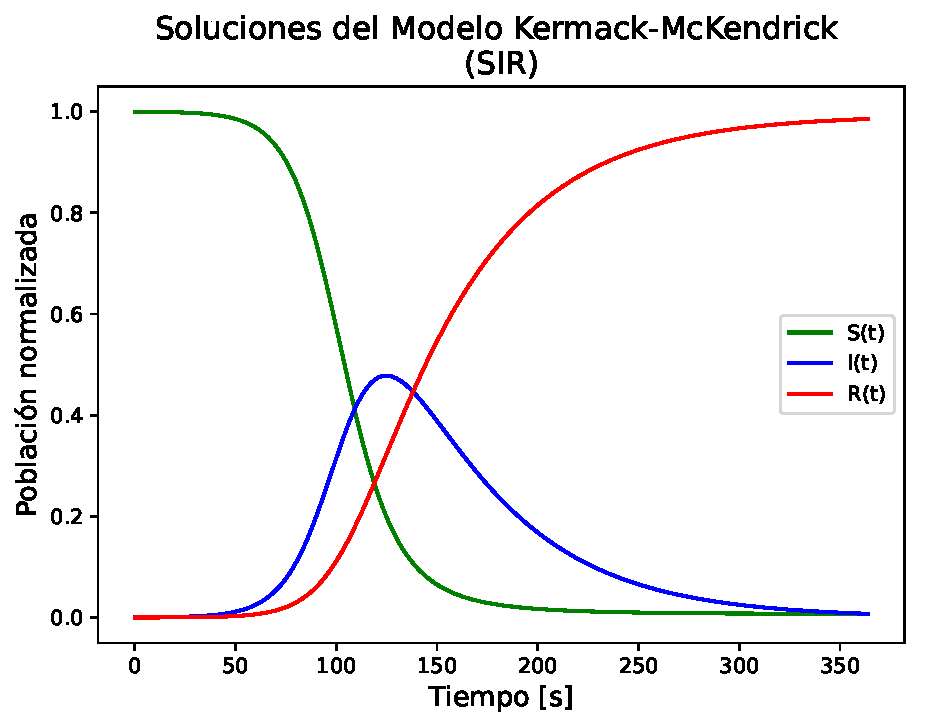
\includegraphics[scale=0.5]{Figuras/f1.pdf}\hspace{0.5cm}
          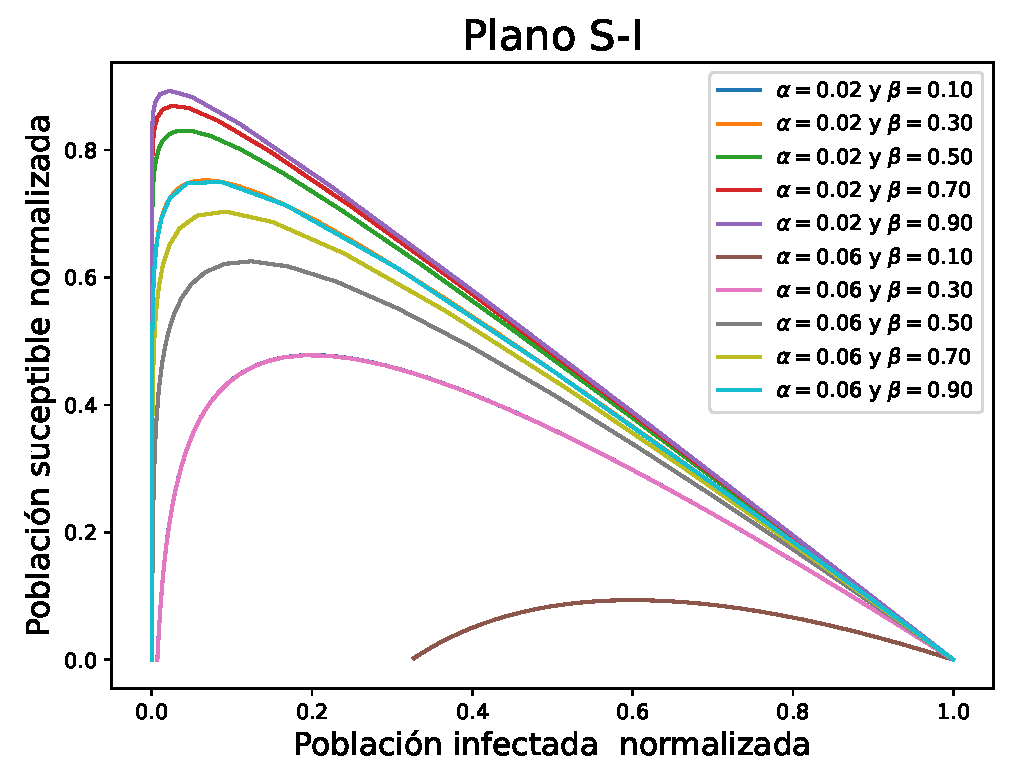
\includegraphics[scale=0.45]{Figuras/f2.pdf}
          \caption{Soluciones del sitema de ecuaciones diferenciales (izquierda). Curvas del plano S-I, variando $\alpha$ y $\beta$ (derecha).}
          \label{fig:1}
      \end{figure*}

    \subsection{estimación del tiempo de recuperación}
    
    Si ya no hay nuevos infecciosos ($\beta SI=0$) entonces 
    
    $$\dot I =-\alpha I$$ $$\Rightarrow \hspace{0.5cm} I(t)=I_0e^{-\alpha t}$$
    $$\Leftrightarrow \hspace{0.5cm} \ln\left(\frac{I(t)}{I_0}\right)=-\alpha t$$
    $$\Leftrightarrow \hspace{0.5cm} \frac{\ln I_0-\ln I(t)}{t}=\alpha $$
    
    En este, caso la probabilidad de ser infeccioso al tiempo $t$ es: 
    
    \begin{equation}\label{eq:6}
        F(t)=1-\frac{I(t)}{I_0}=1-e^{-\alpha t}
    \end{equation}
    
    Entonces la función de densidad de probabilidad es:
    
    \begin{equation}\label{eq:7}
        f(t)=F(t)=\alpha e^{-\alpha t}
    \end{equation}
    
    y la esperanza, que en este caso puede pensarse como el tiempo medio de infección es: 
    
    \begin{equation}\label{eq:8}
        E[X]=\int_{-\infty}^{\infty}tf(t)dt=\int_{-\infty}^{\infty}t\alpha e^{-\alpha t}dt=\frac{1}{\alpha}
    \end{equation}
    
    \subsection{Caso sin remoción}
    
    Suponiendo que los infectados no mueren, pero al curarse son susceptibles de volver a enfermarse (Como una gripe común) se tiene entonces algo del estilo:
    
    \begin{center}
    \hspace{0.4cm}\xymatrix{*+<0.4cm>[F]{S}\ar@/^{8mm}/[r]^{\alpha S} & *+<0.4cm>[F]{I}\ar@/^{8mm}/[l]^{\beta}}    
    \end{center}
    
    En este caso el sistema de ecuaciones es 
    
    \begin{equation}\label{eq:9}
         \tcboxmath[colback=white,colframe=gray, title=Modelo SI]{\begin{array}{ccc}
            \dot S & = & \beta I -\alpha SI \\
            \dot I & = & \alpha SI - \beta I\\            
        \end{array}} 
    \end{equation}
    
    Con
    
    \begin{equation}\label{eq:10}
        N=S(t)+I(t).
    \end{equation}
    
    Tomando $r=\alpha N-\beta$ y $ k=r/\alpha$ se tiene que 
    
    $$\dot I=\alpha SI-\beta I=\alpha (N-I)I-\beta I=\cdots $$ 
    $$\cdots=(\alpha N-\beta)I-\alpha I^2=(\alpha N-\beta)I\left(1-\frac{\alpha}{\alpha N-\beta}I\right)=\cdots$$
    $$\cdots=rI\left(1-\frac{\alpha}{r}I\right)=rI\left(1-\frac{I}{k}\right)$$
    
    i.e. se tiene la ecuación logística
    
    \begin{equation}\label{eq:11}
        \dot I=rI\left(1-\frac{I}{k}\right).
    \end{equation}
    
    Ri $r>0$ entonces $\dot I\leq rI(t) \hspace{0.3cm}\forall t$ por lo que la enfermedad gradualmente desaparece. Si $r>0$ entonces se tiene una epidemia. Considerando que $r=\alpha N-\beta$, estas condiciones se traducen, en términos del número reproductivo básico, en que $R_0=\alpha N/\beta>1$ y  $R_0=\alpha N/\beta<S1$ respectivamente.\\ \newline Para resolver, de la ecuación (\ref{eq:11}) se tiene que:
    
    $$\frac{\frac{dI}{dt}}{I\left(1-\frac{I}{k}\right)}=r$$
    $$\Leftrightarrow \hspace{0.5cm} \int \frac{dI}{I\left(1-\frac{I}{k}\right)}=\int r dt=rt+\zeta_1$$
    $$\Leftrightarrow \hspace{0.5cm} rt+\zeta_1=\int\frac{dI}{I}+\int\frac{dI}{k-I}=\cdots$$ $$\cdots=\ln I- \ln(k-1) + \zeta_2=\ln\left(\frac{I}{k-I}\right)+\zeta_2$$    
    $$\Leftrightarrow \hspace{0.5cm} \frac{I}{k-I}=e^{rt+\zeta_1-\zeta_2}=\underbrace{e^{\zeta_1-\zeta_2}}_{\zeta}e^{rt}$$
    $$\Leftrightarrow \hspace{0.5cm}I=(k-I)\zeta e^{rt}=k\zeta e^{rt}-I\zeta e^{rt}$$  $$\Leftrightarrow \hspace{0.5cm}I(t)=\frac{k \zeta e^{rt}}{\left(1+\zeta e^{rt}\right).}$$
    
   En particular:
   
   $$I_0=I(t=0)=\frac{k\zeta}{1+\zeta}\hspace{0.5cm}\Leftrightarrow\hspace{0.5cm} \zeta=\frac{I_0}{k-I_0}$$
   
   \subsubsection{Caso sin remoción pero con tratamiento de recuperación}

   Inicialmente $\beta$ era la recuperación. Considerando una recuperación de la forma $\overline{\beta}=\beta/(1+I)$, se tiene entonces el sistema:

   \begin{equation}\label{eq:12}
         \tcboxmath[colback=white,colframe=gray, title=Modelo SI]{\begin{array}{ccc}
            \dot S & = & \frac{\beta I}{1+I} I -\alpha SI \\
            \dot I & = & \alpha SI - \frac{\beta I}{1+I}\\            
        \end{array}} 
    \end{equation}

    donde, por la ecuación (\ref{eq:10}) se tiene que 

    \begin{equation}\label{eq:13}
        \dot I=\alpha I(N-I)-\frac{\beta I}{1+I}
    \end{equation}

    cuyas soluciones estacionaras ($\dot I\equiv0$) se obtienen de 

    $$\alpha I(N-I)=\frac{\beta I}{1+I}\hspace{0.5cm}\Leftrightarrow\hspace{0.5cm} (N-I)(1+I)=\frac{\beta I}{\alpha I}=\frac{\beta }{\alpha }$$

    que es una parábola.

    \section{Modelo SIR con demografía.}
    En este caso, se considera que la enfermedad permanece en la población el suficiente tiempo para apreciar los efectos de las tasas naturales de natalidad, $\Lambda$, y de mortalidad, $\mu$. I.e. se tiene un caso de la forma:

    \begin{center}
       \vspace{0.5cm}
       \hspace{0.6cm}\xymatrix{\ar[r]^{\Lambda}&*+<0.6cm>[F]{S} \ar[r]^{\alpha S}+\ar[d]^{\mu} & *+<0.6cm>[F]{I} \ar[r]^{\beta} +\ar[d]^{\mu}&*+<0.6cm>[F]{R} \ar[d]^{\mu}\\&&&}
       \vspace{0.5cm}
    \end{center}

    Con el sistema de ecuaciones diferenciales:

    \begin{equation}\label{eq:14}
         \tcboxmath[colback=white,colframe=gray, title=Modelo SIR con demografía]{\begin{array}{ccl}
            \dot S & = & \Lambda -\alpha SI -\mu S \\
            \dot I & = & \alpha SI - \beta I - \mu I \\
            \dot R & = & \beta I -\mu R\\
        \end{array}} 
    \end{equation}

    En este caso la ecuación (\ref{eq:1}) también es válida sin embargo, se tiene que 

    \begin{equation}\label{eq:15}
        \dot N= \dot I+ \dot S+ \dot R=\Lambda-\mu(\underbrace{S+I+R}_{=N})
    \end{equation}

    Considerando la solución estacionaria ($\dot N\equiv0$), se tiene que $N=\Lambda/\mu$. En particular, cuando $t\to \infty$ debe ocurrir que $N_{\infty}=\Lambda/\mu$\\\newline Como $R$ se puede escribir en términos de $N,I$ y $S$ entonces es redundante (en términos de álgebra lineal, se puede ver como combinación lineal de las otras soluciones). De manera que podemos considerar solo las dos primeras ecuaciones del sistema. Más aún lo consideraremos adimensionalizado. Tomando $\tau=(\alpha+\mu)t$ se tiene que
    
    $$\frac{dS}{d\tau}=\frac{1}{\beta+\mu}\frac{dS}{dt}$$
    $$\frac{dI}{d\tau}=\frac{1}{\beta+\mu}\frac{dI}{dt}$$
    
    y tomando $\displaystyle{x=\frac{\mu}{\Lambda}S}$, $\displaystyle{y=\frac{\mu}{\Lambda} I}$, $\displaystyle{\rho=\frac{\mu}{\beta+\mu}}$ y $\displaystyle{R_0=\frac{\Lambda \alpha}{\mu(\beta+\mu)}}$ se tiene el sistema:

    \begin{equation}\label{eq:16}
    \begin{array}{cl}
         \displaystyle{\frac{dx}{d\tau}}=& (1-x)-R_0xy \\ 
         \displaystyle{\frac{dy}{d\tau}}=& (R_0x-1)y 
    \end{array}  
    \end{equation}

    Encontrando los puntos fijos:

    $$\rho(1-x)-R_0xy=0$$
    $$(R_0x-1)y=0$$

    En el caso en que no hay infectados ($y=0$) necesariamente $x=1$. Por lo que $E_0=(1,0)$ es el equilibrio libre de enfermedad. Si $y\neq 0$ entonces, de la primera ecuación: 

    $$\rho(1-x)=R_0xy\hspace{0.5cm}\Leftrightarrow\hspace{0.5cm}\frac{\rho(1-x)}{R_0x}=y$$

    y de la segunda ecuación, $x=\displaystyle{\frac{1}{R_0}}$, con lo cual:

    $$y=\frac{\rho\left(1-\frac{1}{R_0}\right)}{R_0\frac{1}{R_0}}=\rho\left(1-\frac{1}{R_0}\right)$$

    Con lo que $\displaystyle{E_1=\left(\frac{1}{R_0}, \rho\left(1-\frac{1}{R_0}\right)\right)}$ es un punto de equilibrio. Si $R_0<1\hspace{0.5cm}\Rightarrow\hspace{0.5cm}\left(1-\frac{1}{R_0}\right)<0$ de manera que el punto no es fe asible o de interés biológico. Si $R_0=1$ entonces $E$ se encuentra sobre el eje de los susceptibles, con lo cual no hay infecciosos, por lo que no es un caso interesante. Si $R_0>1$ entonces $E \in (\mathbb{R_+}\times\mathbb{R_+})$ y si es de interés biológico. En este caso se conoce como equilibrio endémico.\\ \newline
    Considerando el cambio de la población infeciosa repecto al cambio de la población susceptible:

    $$\frac{dy}{dx}=\frac{R_0x-1}{(1-x)-R_0xy}=\frac{f(x,y)}{g(x,y)}$$

    Se tienen las cero-clinas $y=0, \displaystyle{y=\frac{\rho(1-x)}{R_0x}}$ y $\displaystyle{x=\frac{1}{R_0}}$. \\\newline

    \textbf{Linealización y un análisis local de los puntos de equilibrio.}\\ \newline Para la  linealizar el sistema (\ref{eq:16}) se toman derivadas parciales respeto a $x $ y $y$. I.e. la matríz jacobiana es tal que 

    $$J_{(X,Y)}=\left(\begin{array}{cc}
       -\rho-R_0y  & -R_0x \\
       R_0y  & R_0x-1
    \end{array}\right)$$

    De manera que en $E_0=(1,0):$
    
    $$J_{E_0}=\left(\begin{array}{cc}
       -\rho  & -R_0 \\
       0 & R_0-1
    \end{array}\right)$$

    Así, el polinomio característico es tal que

    $$p(\lambda)=\det (J_{E_0}-\lambda I)=\det \left(\begin{array}{cc}
       -\rho-\lambda  & -R_0 \\
       0 & R_0-1-\lambda
    \end{array}\right)=\cdots$$
    $$\cdots=(-\rho-\lambda)(R_0-1-\lambda)$$

    con los valores própios $\lambda_1=-\rho<0$ y $\lambda_2=R_0-1$. Si $R_0<1$ entonces $E_0$ es estable asintóticamente. Si $R_0>1$ entonces  $E_0$ es punto silla. \newline En el caso del equilibrio endémico ($R_0<1$):
    
    $$J_{E}=\left(\begin{array}{cc}
       -\rho-R_0y  & -R_0x \\
       R_0Y & 0
    \end{array}\right)\hspace{0.5cm}$$

    con $tra(J_{E})<0$ y $\det(J_E)=R_0^2xy>0$. Esto implíca que $E$ es localmente asintóticamente estable. Haciendo un análisis similar al de $E_0$ se concluye que los valores propios del polinomio característico en este caso son:

    $$\lambda_{1,2}=\rho R_0 \pm \frac{D}{2}\hspace{0.5cm} \textnormal{con} D=(\rho R_0)^2-4\rho(R_0-1)$$

    En este caso, $D>0$ implica que $E$ es un nodo y $D<0$ que es una fuente.
    

    

    

    



    

   
\end{multicols}
    

    




\end{document}
